\documentclass[aspectratio=169]{beamer}

%==================================================
% Packages
%==================================================
\usepackage[french]{babel}
\usepackage[utf8]{inputenc}
\usepackage[T1]{fontenc}

\usepackage{graphicx}
\usepackage{booktabs}
\usepackage{multirow}
\usepackage{amsmath}
\usepackage{tikz}
\usepackage{smartdiagram}
\usepackage{array}
\usepackage{ragged2e}

%==================================================
% Couleurs
%==================================================

\definecolor{ENSPMBlue}{RGB}{0,51,102}
\definecolor{ENSPMGold}{RGB}{255,153,0}
\definecolor{LightGray}{RGB}{245,245,245}

\setbeamercolor{title}{fg=ENSPMBlue}
\setbeamercolor{frametitle}{fg=white,bg=ENSPMBlue}
\setbeamercolor{structure}{fg=ENSPMBlue}
\setbeamercolor{block title}{bg=ENSPMBlue,fg=white}
\setbeamercolor{block body}{bg=LightGray}

\setbeamertemplate{navigation symbols}{}

%==================================================
% Pied de page
%==================================================

\setbeamertemplate{footline}
{
	\leavevmode
	\hbox{
		\begin{beamercolorbox}[wd=.8\paperwidth,ht=2.5ex,dp=1ex,leftskip=0.3cm]{author in head/foot}
			\insertshorttitle
		\end{beamercolorbox}
		
		\begin{beamercolorbox}[wd=.2\paperwidth,ht=2.5ex,dp=1ex,rightskip=0.3cm]{date in head/foot}
			\hfill\insertframenumber/\inserttotalframenumber
		\end{beamercolorbox}
	}
}

%==================================================
% Informations
%==================================================

\title{
	Méthode d'Évaluation des Besoins et\\
	Aide à la Décision Basée sur les Données
}

\author{
	NDZESSA AVELE Bruno Landry
}

\institute{
	École Nationale Supérieure Polytechnique de Maroua
}

\date{\today}

%==================================================
\begin{document}
	%==================================================
	
	%--------------------------------------------------
	\begin{frame}
		\titlepage
	\end{frame}
	
	%--------------------------------------------------
	\begin{frame}{Plan}
		\tableofcontents
	\end{frame}

\section{Introduction}

\begin{frame}{Contexte}
	
	\begin{columns}
		
		\column{0.55\textwidth}
		
		\begin{itemize}
			\item Les décideurs disposent de ressources limitées.
			\item Les besoins exprimés sont nombreux et hétérogènes.
			\item Une mauvaise priorisation conduit à une allocation inefficace.
			\item La Banque Mondiale recommande une démarche structurée d'évaluation des besoins.
		\end{itemize}
		
		\column{0.45\textwidth}
		
		%\includegraphics[width=\linewidth]{images/contexte.png}
		
	\end{columns}
	
\end{frame}

\begin{frame}{Problématique}
	
	\begin{block}{Question de recherche}
		Comment concevoir une méthode permettant :
		
		\begin{enumerate}
			\item d'identifier les besoins prioritaires ;
			\item de segmenter les bénéficiaires ;
			\item d'aider les décideurs à prendre des décisions objectives ?
		\end{enumerate}
		
	\end{block}
	
	\vspace{0.4cm}
	
	\centering
	\Large
	\textbf{Besoins multiples $\Rightarrow$ Décisions complexes}
	
\end{frame}

\begin{frame}{Objectifs}
	
	\begin{block}{Objectif général}
		
		Concevoir une méthode d'aide à la décision fondée sur
		l'évaluation systématique des besoins.
		
	\end{block}
	
	\vspace{0.3cm}
	
	\begin{block}{Objectifs spécifiques}
		
		\begin{itemize}
			\item Collecter les besoins.
			\item Segmenter les populations.
			\item Construire une typologie.
			\item Prioriser les interventions.
			\item Produire des recommandations décisionnelles.
		\end{itemize}
		
	\end{block}
	
\end{frame}

\section{Méthodologie}

\begin{frame}{Méthodologie Adoptée}
	
	\centering
	
	\smartdiagramset{
		uniform color list=ENSPMBlue for 6 items,
		back arrow disabled=true
	}
	
	\smartdiagram[circular diagram]{
		Collecte,
		Prétraitement,
		ACM,
		CAH,
		Typologie,
		Décision
	}
	
\end{frame}

\section{Données}

\begin{frame}{Description des données}
	
	\begin{table}
		\centering
		\begin{tabular}{lll}
			\toprule
			Variable & Type & Description\\
			\midrule
			Age & Quantitative & Age du répondant\\
			Sexe & Qualitative & Homme/Femme\\
			Besoin & Qualitative & Type de besoin\\
			Priorité & Ordinale & Niveau d'urgence\\
			\bottomrule
		\end{tabular}
	\end{table}
	
\end{frame}

\section{Modélisation}

\begin{frame}{Construction de la typologie}
	
	\begin{columns}
		
		\column{0.5\textwidth}
		
		\begin{block}{Analyse Factorielle}
			\begin{itemize}
				\item Réduction dimensionnelle
				\item Visualisation des profils
				\item Détection des associations
			\end{itemize}
		\end{block}
		
		\column{0.5\textwidth}
		
		\begin{block}{Classification}
			\begin{itemize}
				\item CAH sur les coordonnées ACM
				\item Segmentation homogène
				\item Construction des profils
			\end{itemize}
		\end{block}
		
	\end{columns}
	
\end{frame}

\section{Résultats}

\begin{frame}{Résultats Principaux}
	
	\begin{columns}
		
		\column{0.55\textwidth}
		
		\begin{itemize}
			\item 4 groupes identifiés.
			\item Segmentation cohérente.
			\item Profils interprétables.
			\item Priorités d'intervention définies.
		\end{itemize}
		
		\column{0.45\textwidth}
		
		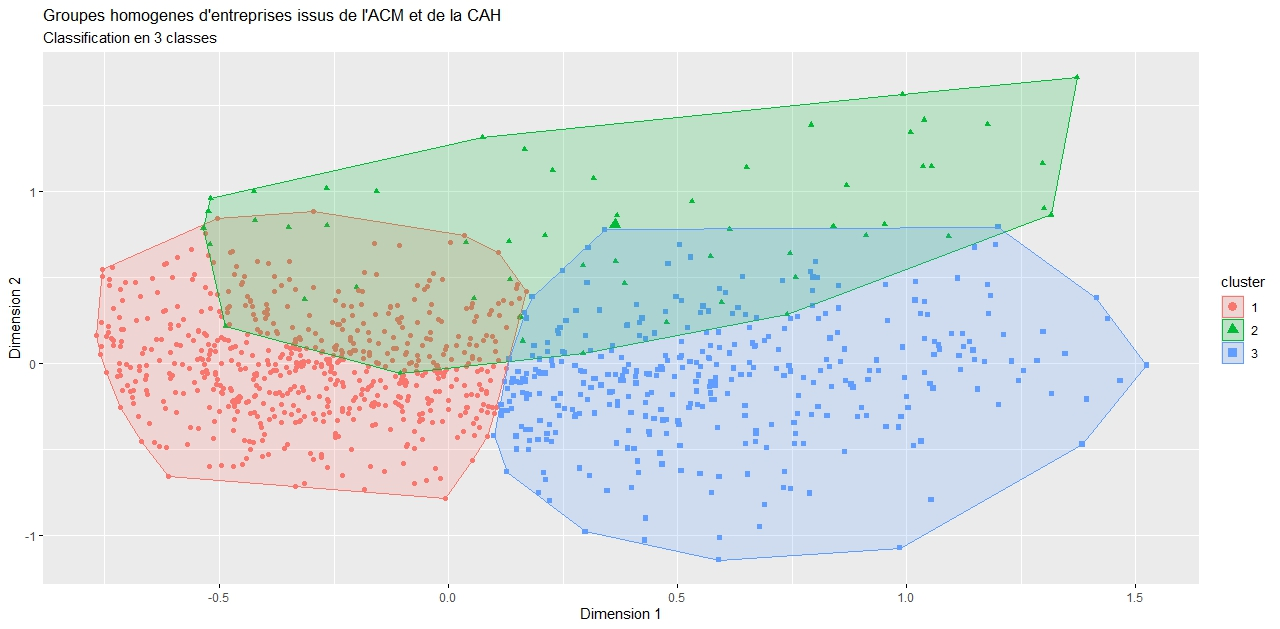
\includegraphics[width=\linewidth]{CAH.jpeg}
		
	\end{columns}
	
\end{frame}

\begin{frame}{Contributions}
	
	\begin{block}{Contributions scientifiques}
		
		\begin{itemize}
			\item Formalisation d'une démarche d'évaluation des besoins.
			\item Construction d'une typologie des bénéficiaires.
			\item Validation par ACM et CAH.
		\end{itemize}
		
	\end{block}
	
	\begin{block}{Contributions techniques}
		
		\begin{itemize}
			\item Développement d'une plateforme web.
			\item Génération automatique de recommandations.
			\item Visualisation interactive des résultats.
		\end{itemize}
		
	\end{block}
	
\end{frame}

\begin{frame}{Architecture de la solution}
	
	\centering
	
	\begin{tikzpicture}[node distance=2cm]
		
		\node (data) [draw, rounded corners] {Base de données};
		
		\node (algo) [draw, rounded corners, right=of data]
		{ACM + CAH};
		
		\node (web) [draw, rounded corners, right=of algo]
		{Application Django};
		
		\draw[->,thick] (data)--(algo);
		\draw[->,thick] (algo)--(web);
		
	\end{tikzpicture}
	
\end{frame}

\section{Conclusion}

\begin{frame}{Conclusion et Perspectives}
	
	\begin{block}{Conclusion}
		
		\begin{itemize}
			\item Les besoins ont été identifiés et structurés.
			\item Une typologie pertinente a été obtenue.
			\item L'approche facilite la prise de décision.
		\end{itemize}
		
	\end{block}
	
	\begin{block}{Perspectives}
		
		\begin{itemize}
			\item Intégration de nouvelles données.
			\item Recommandation basée IA.
			\item Tableau de bord décisionnel avancé.
		\end{itemize}
		
	\end{block}
	
\end{frame}

\begin{frame}
	
	\centering
	
	\vspace{2cm}
	
	{\Huge Merci pour votre attention}
	
	\vspace{1cm}
	
	{\Large Questions ?}
	
\end{frame}

\end{document}
